% Template for Elsevier CRC journal article
% version 1.2 dated 09 May 2011

% This file (c) 2009-2011 Elsevier Ltd.  Modifications may be freely made,
% provided the edited file is saved under a different name

% This file contains modifications for Nuclear Physics B Proceedings Supplement

% Changes since version 1.1
% - added "procedia" option compliant with ecrc.sty version 1.2a
%   (makes the layout approximately the same as the Word CRC template)
% - added example for generating copyright line in abstract

%-----------------------------------------------------------------------------------

%% This template uses the elsarticle.cls document class and the extension package ecrc.sty
%% For full documentation on usage of elsarticle.cls, consult the documentation "elsdoc.pdf"
%% Further resources available at http://www.elsevier.com/latex

%-----------------------------------------------------------------------------------

%%%%%%%%%%%%%%%%%%%%%%%%%%%%%%%%%%%%%%%%%%%%%%%%%%%%%%%%%%%%%%
%%%%%%%%%%%%%%%%%%%%%%%%%%%%%%%%%%%%%%%%%%%%%%%%%%%%%%%%%%%%%%
%%                                                          %%
%% Important note on usage                                  %%
%% -----------------------                                  %%
%% This file should normally be compiled with PDFLaTeX      %%
%% Using standard LaTeX should work but may produce clashes %%
%%                                                          %%
%%%%%%%%%%%%%%%%%%%%%%%%%%%%%%%%%%%%%%%%%%%%%%%%%%%%%%%%%%%%%%
%%%%%%%%%%%%%%%%%%%%%%%%%%%%%%%%%%%%%%%%%%%%%%%%%%%%%%%%%%%%%%

\documentclass[3p,times,procedia]{elsarticle}
\usepackage{nupha_ecrc}


\newcommand{\pp}{pp}
\newcommand{\mpp}{\mathrm{pp}}
\newcommand{\sqrts}{\sqrt{s}}
\newcommand{\lsim}{\,{\buildrel < \over {_\sim}}\,}
\newcommand{\gsim}{\,{\buildrel > \over {_\sim}}\,}
\newcommand{\av}[1]{\left\langle #1 \right\rangle}
\newcommand{\eV}{\mathrm{eV}}
\newcommand{\keV}{\mathrm{keV}}
\newcommand{\MeV}{\mathrm{MeV}}
\newcommand{\GeV}{\mathrm{GeV}}
\newcommand{\TeV}{\mathrm{TeV}}
\newcommand{\ev}{\mathrm{eV}}
\newcommand{\kev}{\mathrm{keV}}
\newcommand{\mev}{\mathrm{MeV}}
\newcommand{\gev}{\mathrm{GeV}}
\newcommand{\gevc}{\mathrm{GeV}/c}
\newcommand{\tev}{\mathrm{TeV}}
\newcommand{\fm}{\mathrm{fm}}
\newcommand{\mm}{\mathrm{mm}} 
\newcommand{\cm}{\mathrm{cm}}
\newcommand{\m}{\mathrm{m}}
\newcommand{\mum}{\mathrm{\mu m}}
\newcommand{\s}{\mathrm{s}}
\newcommand{\ns}{\mathrm{ns}}
\newcommand{\mrad}{\mathrm{mrad}}
\newcommand{\mb}{\mathrm{mb}}
\newcommand{\mub}{\mathrm{\mu b}}
\newcommand{\T}{\mathrm{T}}
\newcommand{\PbPb}{\mbox{Pb--Pb}}
\newcommand{\pt}{p_{\rm T}}
\newcommand{\dNdy}{{\rm d}N_{ch}/{\rm d}y}
\newcommand{\momwin}{[$p$, $p$+$\Delta$ $p$]}
\newcommand{\DtoKpi}{{\rm D}^0 \to {\rm K}^-\pi^+}
\newcommand{\DtoKpipi}{{\rm D}^+\to {\rm K}^-\pi^+\pi^+}
\newcommand{\DstartoDpi}{{\rm D}^{*+} \to {\rm D}^0 \pi^+}
\newcommand{\DstartoDpiPrecise}{{\rm D^{*+}(2010)\to D^0\pi^+}}
\newcommand{\LctopKzeros}{{\rm \Lambda_{c}^+ \to pK^{0}_{s} \to p\pi^+\pi^-}}
\newcommand{\Dstophip}{{\rm D_{s}^+ \to \phi \pi^+ \to K^{+}K^{-} \pi^+}}
\newcommand{\Dzero}{{\rm D^0}}
\newcommand{\Dzerobar}{\overline{{\rm D^0}}}
\newcommand{\Dstar}{{\rm D^{*+}}}
\newcommand{\Dstarm}{{\rm D^{*-}}}
\newcommand{\Dplus}{{\rm D^+}}
\newcommand{\Dminus}{{\rm D^-}}
\newcommand{\Ds}{{\rm D_{s}^+}}
\newcommand{\Dsminus}{{\rm D_{s}^-}}
\newcommand{\Lc}{{\rm \Lambda_{c}^+}}
\newcommand{\Lcminus}{{\rm \Lambda_{c}^-}}
%\newcommand{\ccbar}{${\rm c}\bar{\rm c}$~}
\newcommand{\nbinv}{{\rm nb^{-1}}}
\newcommand{\decleng}{{\rm L}_{xyz}}
\newcommand{\dEdx}{{\rm d}E/{\rm d}x}
\newcommand{\Pv}{{\rm P}_{\rm v}}
\newcommand{\cubar}{{\rm c}\bar{\rm u}}
\newcommand{\cdbar}{{\rm c}\bar{\rm d}}
\newcommand{\mur}{\mu_{\rm R}}
\newcommand{\muf}{\mu_{\rm F}}
\newcommand{\mc}{m_{\rm c}}
\newcommand{\sigmatot}{\sigma_{\rm tot}}
\newcommand{\ccbar}{${\rm c}\bar{\rm c}$~}
\newcommand{\bbbar}{${\rm b}\bar{\rm b}$~}
\newcommand{\Jpsi}{{\rm J}/\psi}
\newcommand{\RAA}{\rm R_{AA}}

\newcommand{\Ntrk}{N_{\rm tracklets}}
\newcommand{\Nvzero}{N_{\rm VZERO}}
\newcommand{\dNdEta}{{\rm d}N_{\rm ch}/{\rm d}\eta}
\newcommand{\dNdpt}{{\rm d}N^{\rm D}/{\rm d}\pt}
\newcommand{\dNDzdpt}{{\rm d}N^{\rm \Dzero}/{\rm d}\pt}
\newcommand{\dNdydpt}{{\rm d}^2N^{\rm D}/{\rm d}y {\rm d}\pt}
\newcommand{\dNDzdydpt}{{\rm d}^2N^{\rm \Dzero}/{\rm d}y {\rm d}\pt}
\newcommand{\fB}{f_{\rm B}}


\newcommand{\ptjet}{{p}^{\tn{jet ch}}_{\tn{T}}}
\newcommand{\pthf}{{p}_\tn{T}^\tn{HF}}
\newcommand{\etajet}{{\eta}_{\tn{jet}}}
\newcommand{\zch}{{z_{\parallel}^{\tn{ch}}}}
\newcommand{\zchr}{{z_{\parallel\tn{, rec.}}^{\tn{ch}}}}
\newcommand{\zchg}{{z_{\parallel\tn{, gen.}}^{\tn{ch}}}}
\newcommand{\pchjet}{{\bm{p}}^\tn{jet ch}}

\newcommand{\ptjchr}{p_\tn{T, rec.}^\tn{jet ch}}
\newcommand{\ptjchg}{p_\tn{T, gen.}^\tn{jet ch}}
\newcommand{\pth}{p_\tn{T}^\tn{h}}

\newcommand{\tn}[1]{\textnormal{#1}} % normal (upright non-bold) text
\newcommand{\dd}{\mathrm{d}} % total differential symbol

%% The ecrc package defines commands needed for running heads and logos.
%% For running heads, you can set the journal name, the volume, the starting page and the authors

%% set the volume if you know. Otherwise `00'
\volume{00}

%% set the starting page if not 1
\firstpage{1}

%% Give the name of the journal
\journalname{Nuclear Physics A}

%% Give the author list to appear in the running head
%% Example \runauth{C.V. Radhakrishnan et al.}
\runauth{}

%% The choice of journal logo is determined by the \jid and \jnltitlelogo commands.
%% A user-supplied logo with the name <\jid>logo.pdf will be inserted if present.
%% e.g. if \jid{yspmi} the system will look for a file yspmilogo.pdf
%% Otherwise the content of \jnltitlelogo will be set between horizontal lines as a default logo

%% Give the abbreviation of the Journal.
\jid{nupha}

%% Give a short journal name for the dummy logo (if needed)
\jnltitlelogo{Nuclear Physics A}

%% Hereafter the template follows `elsarticle'.
%% For more details see the existing template files elsarticle-template-harv.tex and elsarticle-template-num.tex.

%% Elsevier CRC generally uses a numbered reference style
%% For this, the conventions of elsarticle-template-num.tex should be followed (included below)
%% If using BibTeX, use the style file elsarticle-num.bst

%% End of ecrc-specific commands
%%%%%%%%%%%%%%%%%%%%%%%%%%%%%%%%%%%%%%%%%%%%%%%%%%%%%%%%%%%%%%%%%%%%%%%%%%

%% The amssymb package provides various useful mathematical symbols
\usepackage{amssymb}
%% The amsthm package provides extended theorem environments
%% \usepackage{amsthm}

%% The lineno packages adds line numbers. Start line numbering with
%% \begin{linenumbers}, end it with \end{linenumbers}. Or switch it on
%% for the whole article with \linenumbers after \end{frontmatter}.
%% \usepackage{lineno}

%% natbib.sty is loaded by default. However, natbib options can be
%% provided with \biboptions{...} command. Following options are
%% valid:

%%   round  -  round parentheses are used (default)
%%   square -  square brackets are used   [option]
%%   curly  -  curly braces are used      {option}
%%   angle  -  angle brackets are used    <option>
%%   semicolon  -  multiple citations separated by semi-colon
%%   colon  - same as semicolon, an earlier confusion
%%   comma  -  separated by comma
%%   numbers-  selects numerical citations
%%   super  -  numerical citations as superscripts
%%   sort   -  sorts multiple citations according to order in ref. list
%%   sort&compress   -  like sort, but also compresses numerical citations
%%   compress - compresses without sorting
%%
%% \biboptions{comma,round}

% \biboptions{}

% if you have landscape tables
\usepackage[figuresright]{rotating}

% put your own definitions here:
%   \newcommand{\cZ}{\cal{Z}}
%   \newtheorem{def}{Definition}[section]
%   ...

% add words to TeX's hyphenation exception list
%\hyphenation{author another created financial paper re-commend-ed Post-Script}

% declarations for front matter

\begin{document}

\begin{frontmatter}

%% Title, authors and addresses

%% use the tnoteref command within \title for footnotes;
%% use the tnotetext command for the associated footnote;
%% use the fnref command within \author or \address for footnotes;
%% use the fntext command for the associated footnote;
%% use the corref command within \author for corresponding author footnotes;
%% use the cortext command for the associated footnote;
%% use the ead command for the email address,
%% and the form \ead[url] for the home page:
%%
%% \title{Title\tnoteref{label1}}
%% \tnotetext[label1]{}
%% \author{Name\corref{cor1}\fnref{label2}}
%% \ead{email address}
%% \ead[url]{home page}
%% \fntext[label2]{}
%% \cortext[cor1]{}
%% \address{Address\fnref{label3}}
%% \fntext[label3]{}

%% Instructions from Editor: Please use the following \dochead only in the preprint version (e-print arXiv etc.); 
%% use empty \dochead{} when submitting to Nuclear Physics A!
\dochead{XXVIIIth International Conference on Ultrarelativistic Nucleus-Nucleus Collisions\\ (Quark Matter 2019)}
%\dochead{}
%% Use \dochead if there is an article header, e.g. \dochead{Short communication}
%% \dochead can also be used to include a conference title, if directed by the editors
%% e.g. \dochead{17th International Conference on Dynamical Processes in Excited States of Solids}

\title{}

%% use optional labels to link authors explicitly to addresses:
%% \author[label1,label2]{<author name>}
%% \address[label1]{<address>}
%% \address[label2]{<address>}

\author{}

\address{}

\begin{abstract}
The measurement of heavy-flavour production represents a powerful tool to study the medium formed in high-energy 
heavy-ion collisions. Produced in hard scattering processes on a timescale shorter than the QGP formation time, 
they experience the whole evolution of the medium interacting with its constituents. The measurements of charm-hadron 
production allows testing the mechanisms of in-medium parton energy loss. Moreover, the study of charm-baryon 
production in heavy-ion collisions and in particular the baryon-to-meson ratio, provides unique information on 
hadronisation mechanisms, constraining the role of coalescence and testing the predicted presence of diquark states in the medium.
In this contribution, the ALICE results on open charmed meson and baryon production with the 2018 PbPb sample will be presented
with a focus on the recent measurements of $\Lc$/$\Dzero$ and $\Ds$/$\Dzero$ ratios as a function of transverse momentum in central and peripheral PbPb 
collisions and as a function of charged particle multiplicity and transverse momentum in proton-proton collisions. 
Next exploratory measurements of strange charmed baryons production and baryon production in jets will also be discussed.
\end{abstract}

\begin{keyword}
Heavy ions \sep heavy flavours \sep energy loss \sep quark recombination
\end{keyword}
\end{frontmatter}

%%
%% Start line numbering here if you want
%%
% \linenumbers

%% main text
\section{Introduction}
\label{intro}
Charm and beauty quarks are produced in hard scattering processes at the very early stages of heavy-ion collisions. As a consequence of the 
large momentum trasferred in these processes, their production can be effectively described by perturbative QCD calculations. 
Once produced, they traverse the hot and dense medium and they interact with the medium constituens via inelastic or elastic processes.
Therefore, by studying their suppression in heavy-ion collisions, one can investigate the microscopic nature of energy loss processes
and constrain fundamental parameters of the system, like the charm diffusion coefficient. On the other side, measurements of 
heavy-flavour hadrochemistry can be used to constrain the relevance of processes of quark recombination in the medium. A quantitative 
understanding of heavy-flavour recombination is indeed extremely important to characterise the nature of quasi-particles in the QGP.
The study of heavy-flavour production can also play an important role in understanding the nature of the system we create in proton-proton and 
proton-lead collisions. The study of hadron ratios in these systems can indeed highight the presence of recombination 
processes in small systems and shed new lights into the medium-like phenomena that have been observed in the last years both at RHIC and at the LHC. 

\section{Heavy-quark energy loss}
\label{intro}
With the large statistics collected at the end of 2018, ALICE was able to update its measurement of the nuclear modification factor of 
$\Dzero$ mesons in central and peripheral PbPb collisions. In Fig.~\ref{fig:prompt_nonpromptRAA} (left), the $\RAA$ of $\Dzero$ in the centrality 
interval 0--10$\%$ is presented as a function of the trasnverse momentum $\pt$. For the first time at the LHC, the $\Dzero$ production is measured 
in central collisions down to 0 GeV/c. The high accuracity of this measurement is now capable of challenging theoretical calculation in a wide 
transverse momentum region. In particular, the new 0--1 $\GeV$ interval seems to confirm the relevance of shadowing mechanisms for charm at low $\pt$
which reduce the charm production in the low-$x$ region. A new measurement of the beauty suppression via the analysis of non-prompt $\Dzero$ hadrons 
was also presented. In the middle panel of Fig.~\ref{fig:prompt_nonpromptRAA}, the ratio of the $\RAA$ of prompt and non-prompt $\Dzero$ mesons is presented
as a function of $\pt$. The ratio shows a maximum for $\pt$ of about 10 $\GeV$ and a decrease at higher transverse momenta. This trend is pretty well 
described by theoretical calculations which include a different relevance of energy loss mechanisms for charm and beauty quark. 
This new measurement is therefore consistent with the expectation of flavour dependence of the mechanisms of energy loss in presence of free color charges.

\begin{figure}[h]
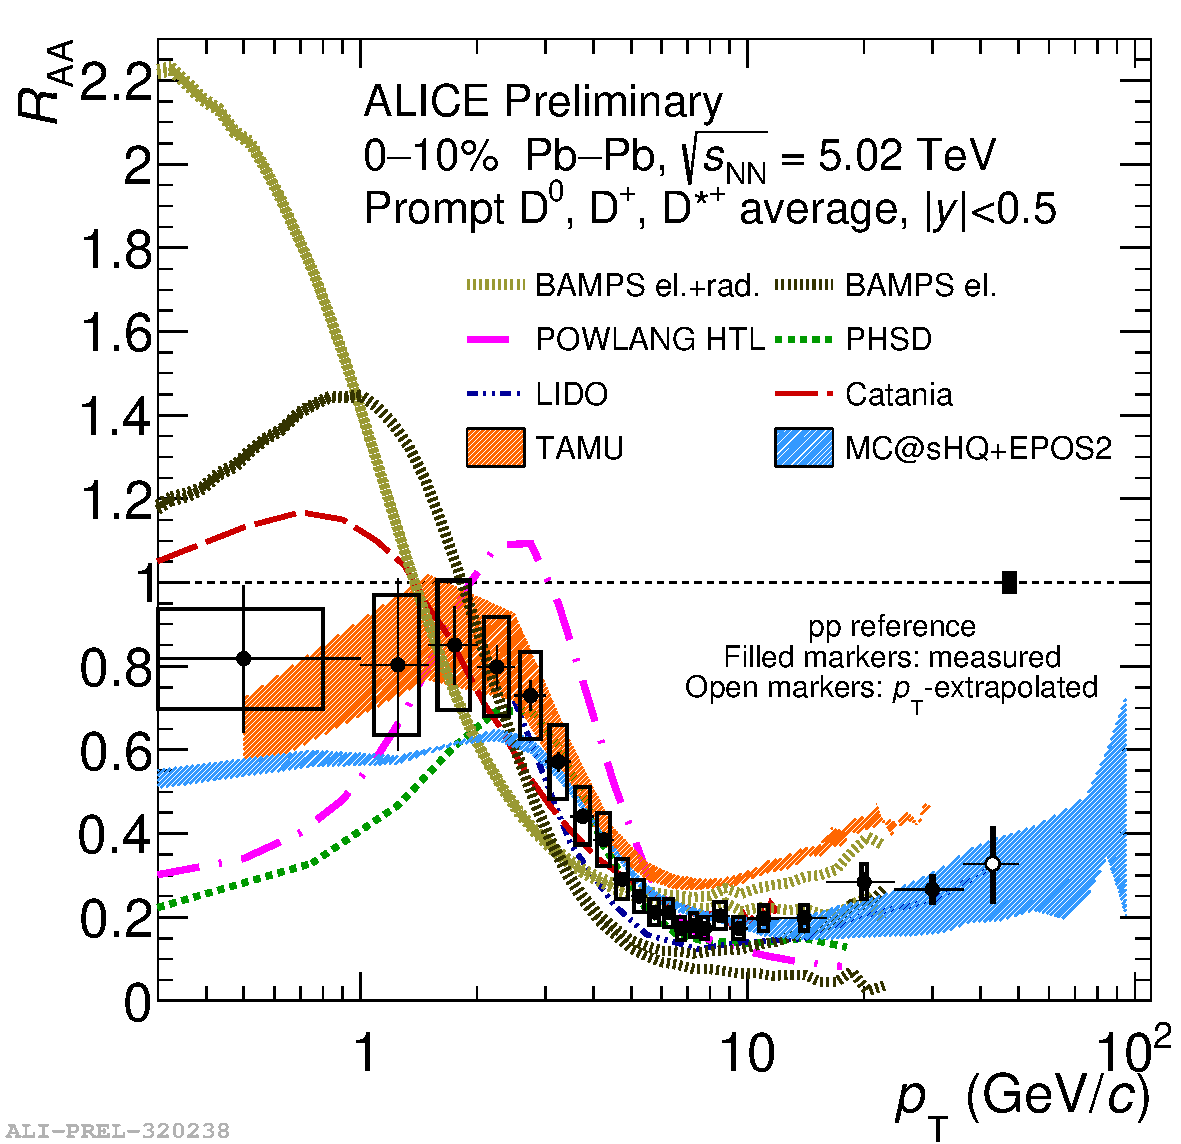
\includegraphics[width=0.33\textwidth]{Plots/D/2019-10-31-2019-10-28-DmesonAverage_vs_transportmodels_010_5dot02.pdf}
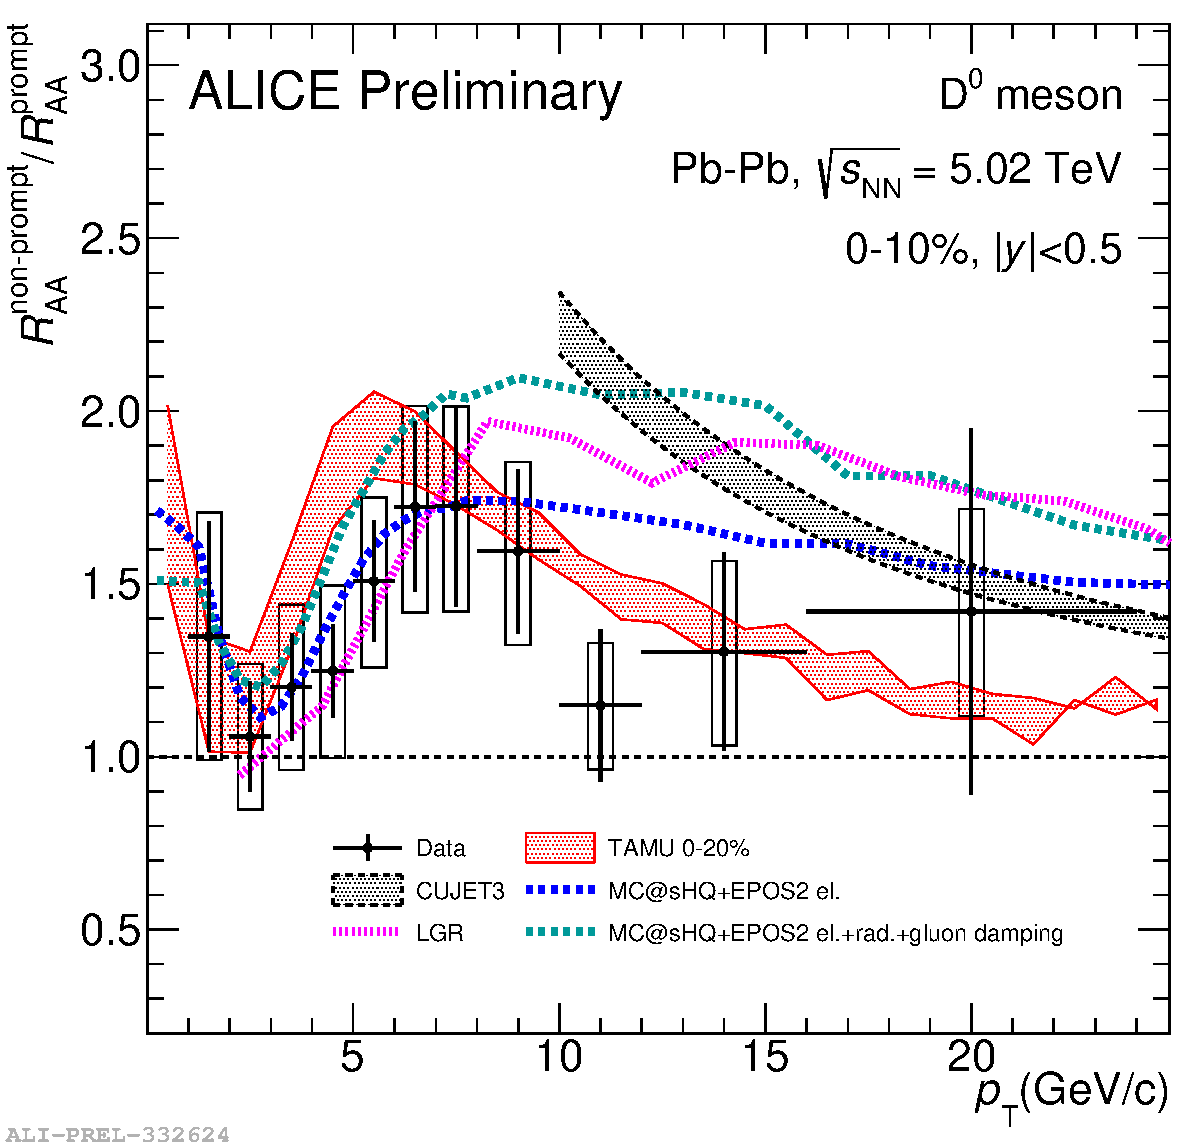
\includegraphics[width=0.33\textwidth]{Plots/NP/2019-10-31-2019-10-29-D0PbPb5TeV_010_RaaRatio_wModel.pdf}
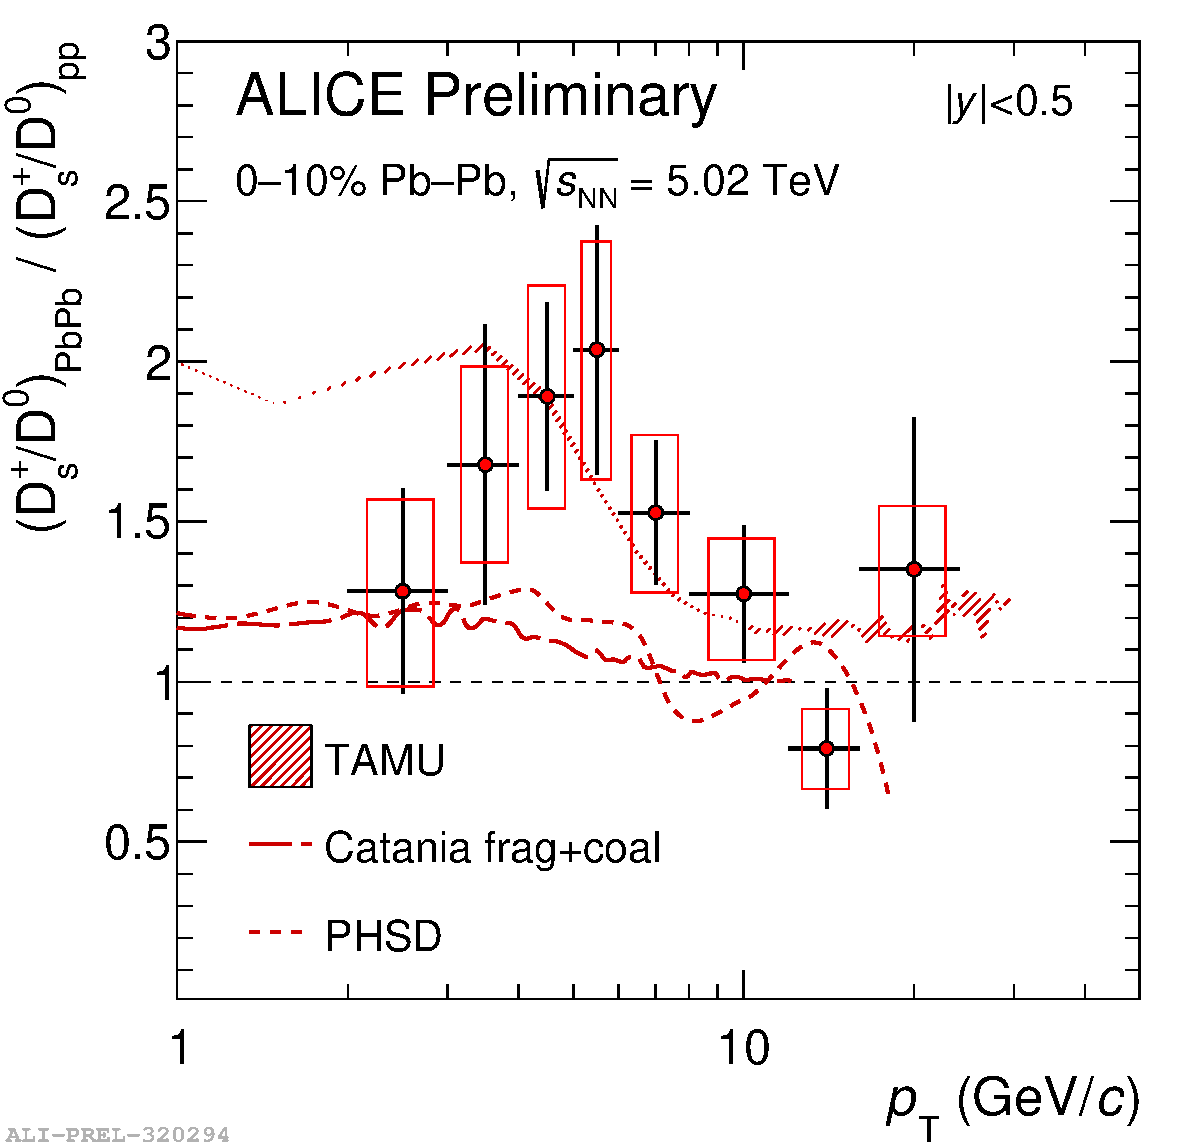
\includegraphics[width=0.33\textwidth]{Plots/D/2019-10-31-2019-10-28-DoubleRatio_DsOverDzero_PbPb2018_010_pp_WithModels.pdf}
\caption{Alleluja}
\label{fig:prompt_nonpromptRAA}
\end{figure}

\begin{figure}[h]
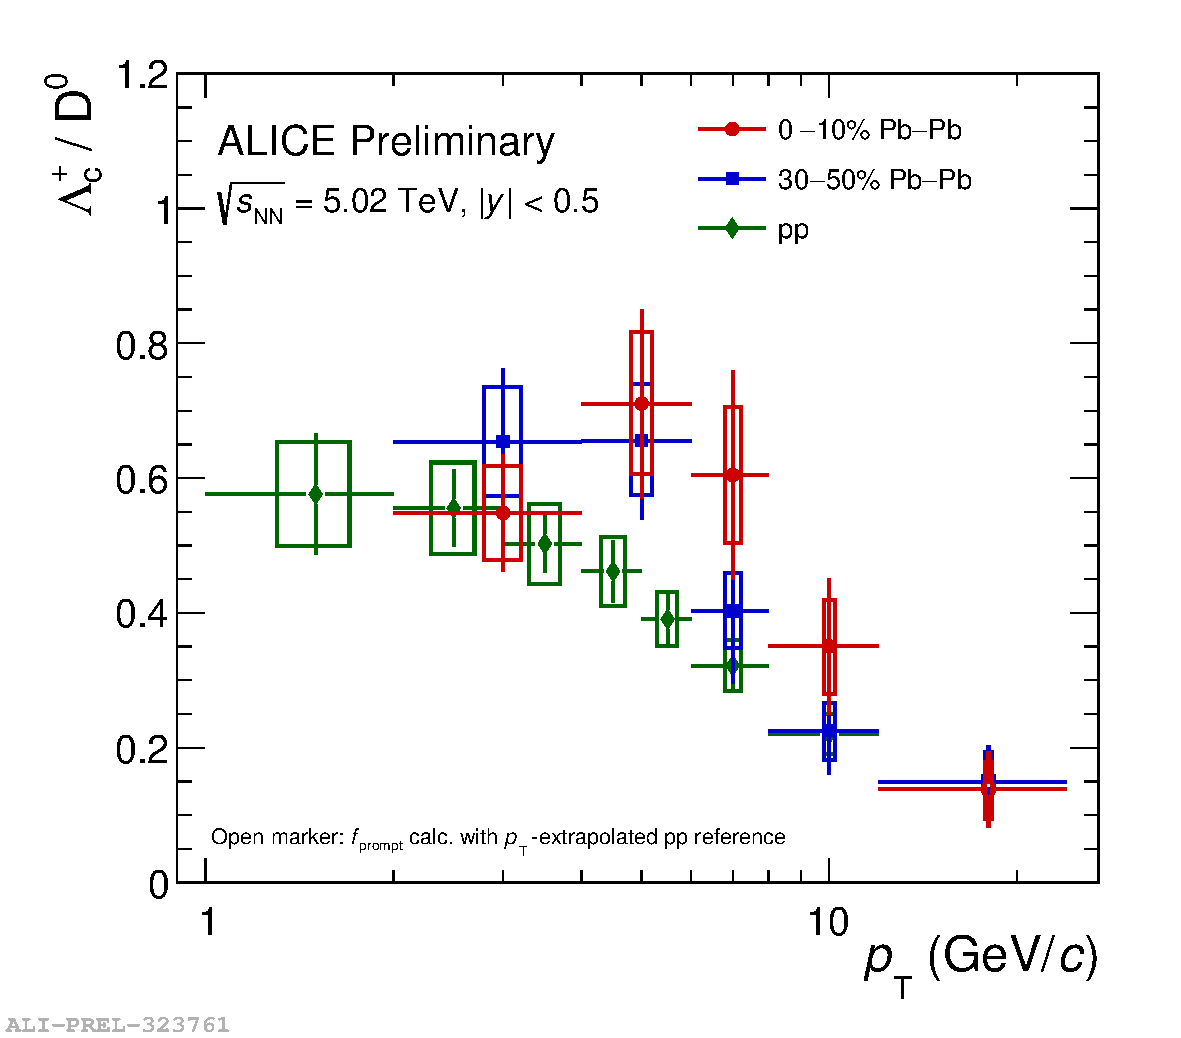
\includegraphics[width=0.49\textwidth]{Plots/PbPbLc/2019-10-28-LcD_PbPb18_010_3050_pp_Logx_shift.pdf}
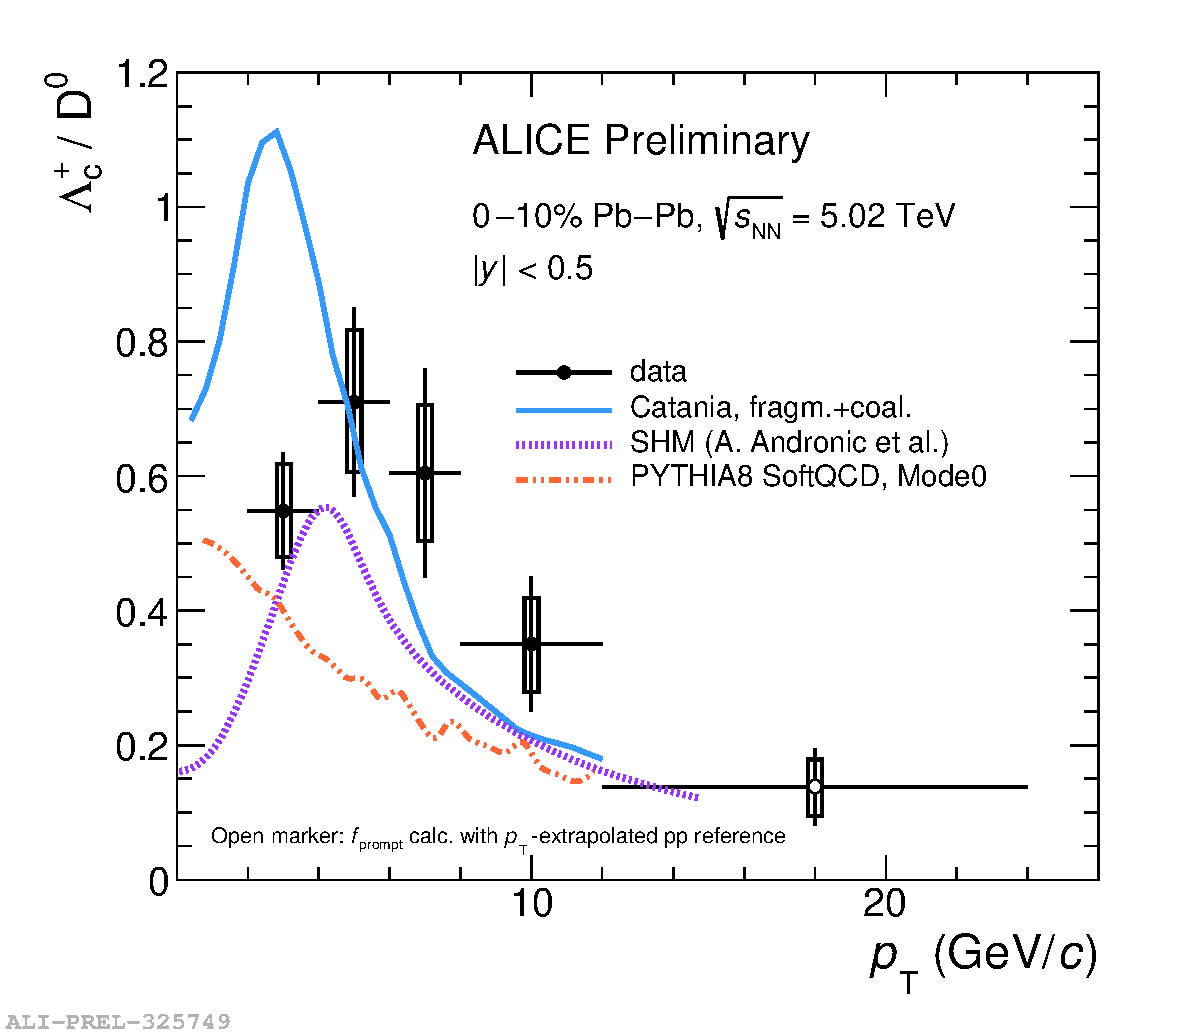
\includegraphics[width=0.49\textwidth]{Plots/PbPbLc/2019-10-31-LcD_PbPb18_010_theory_withPythia.pdf}
\caption{Alleluja}
\label{fig:LcD0andtheory}
\end{figure}

\begin{figure}[h]
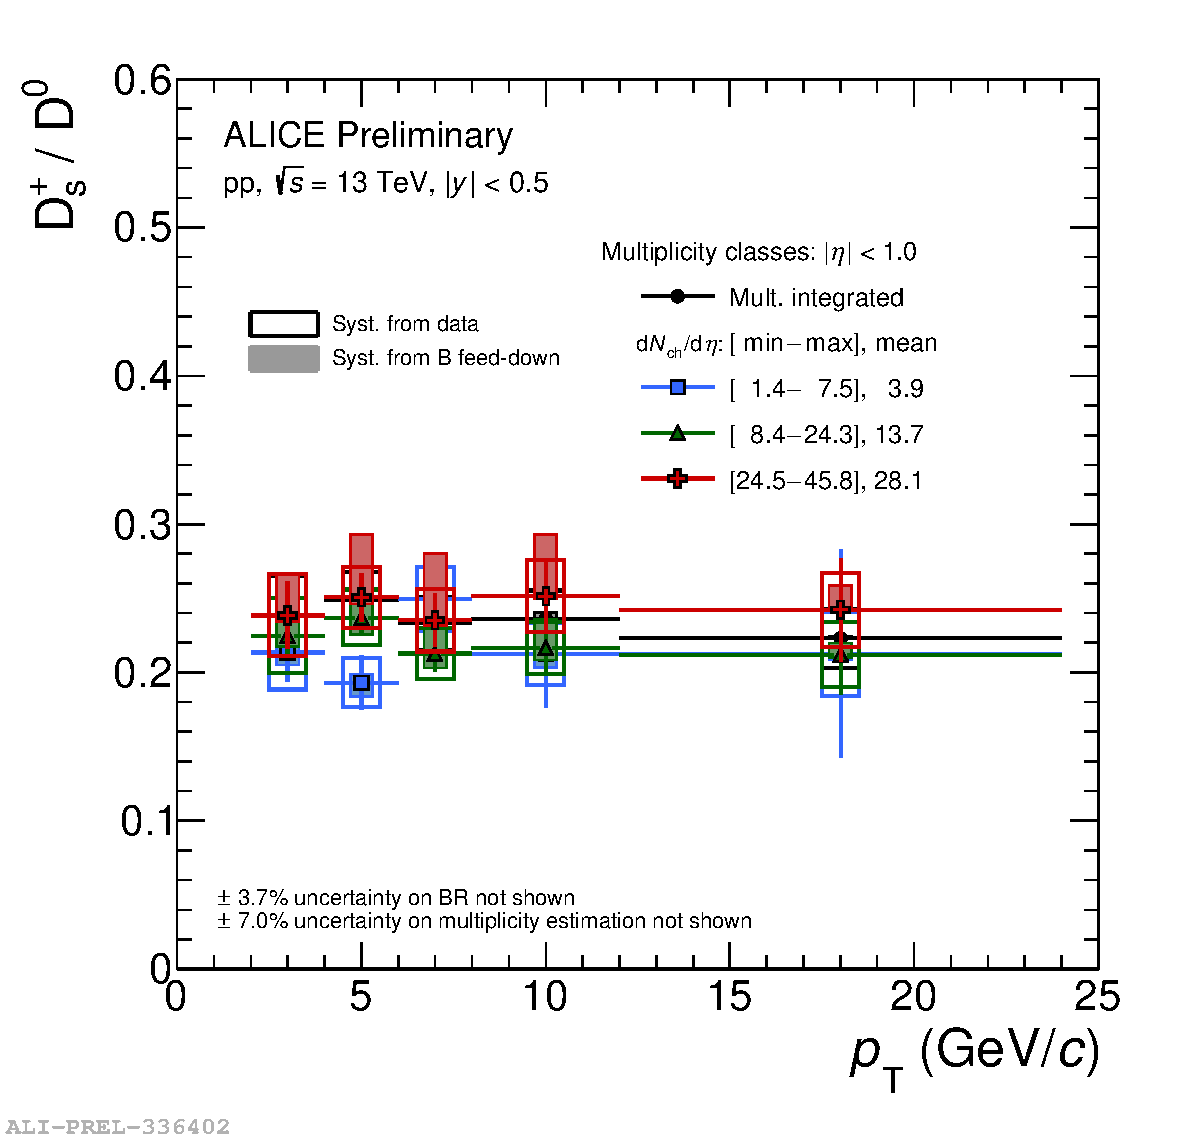
\includegraphics[width=0.49\textwidth]{Plots/ppHM/2019-10-31-2019-10-31-DsOverD0_allMult_MB.pdf}
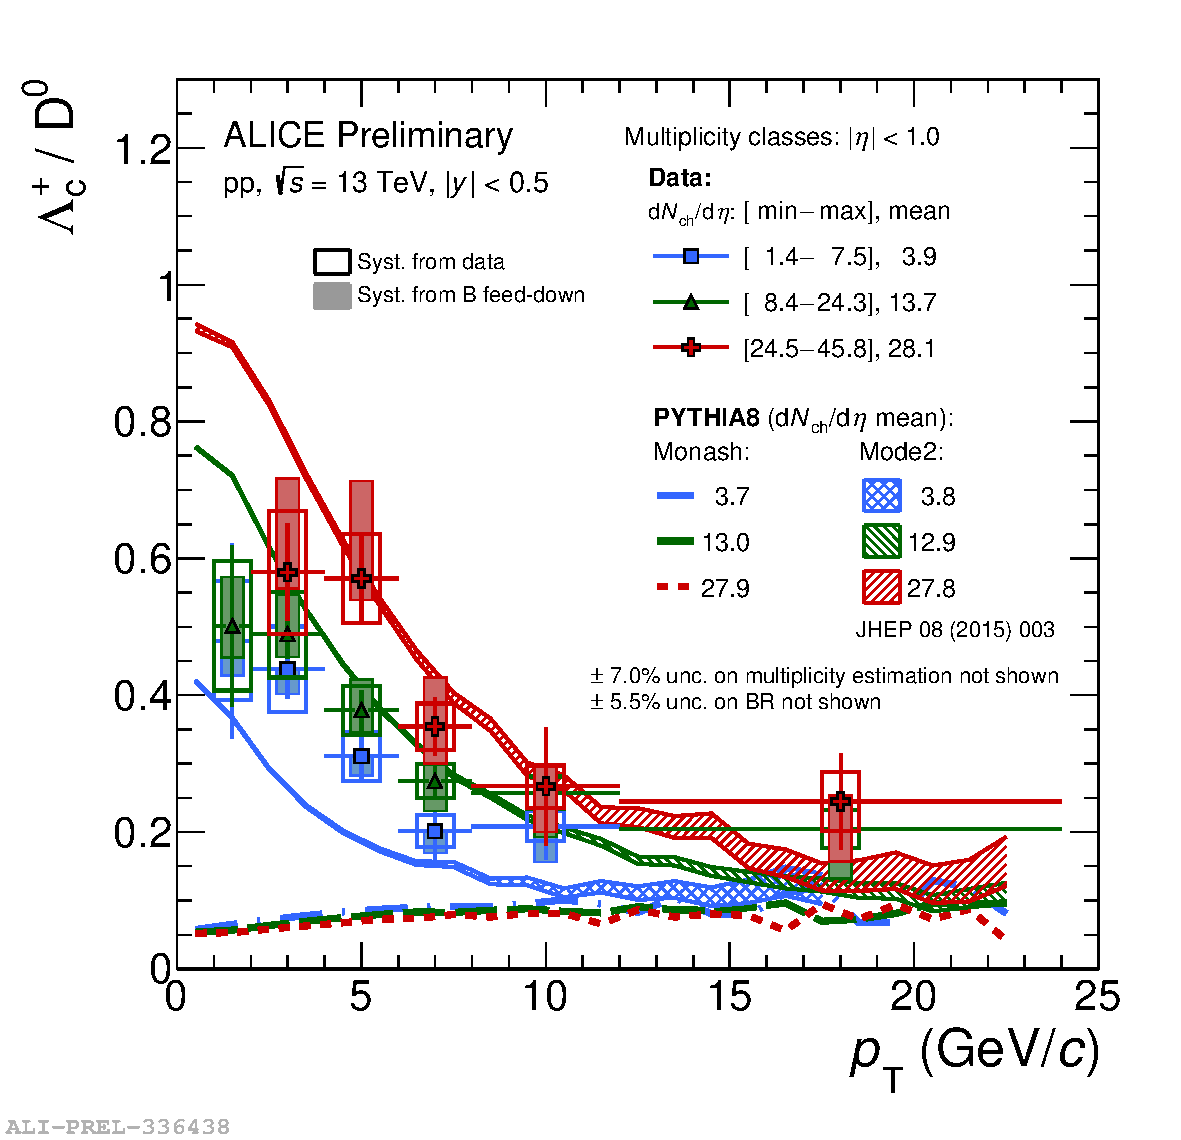
\includegraphics[width=0.49\textwidth]{Plots/ppHM/2019-10-31-2019-10-31-LcpKpiOverD0_wPythiaMonashMode2_allMult.pdf}
\caption{Alleluj sdsda}
\label{fig:highmult}
\end{figure}

\begin{figure}[h]
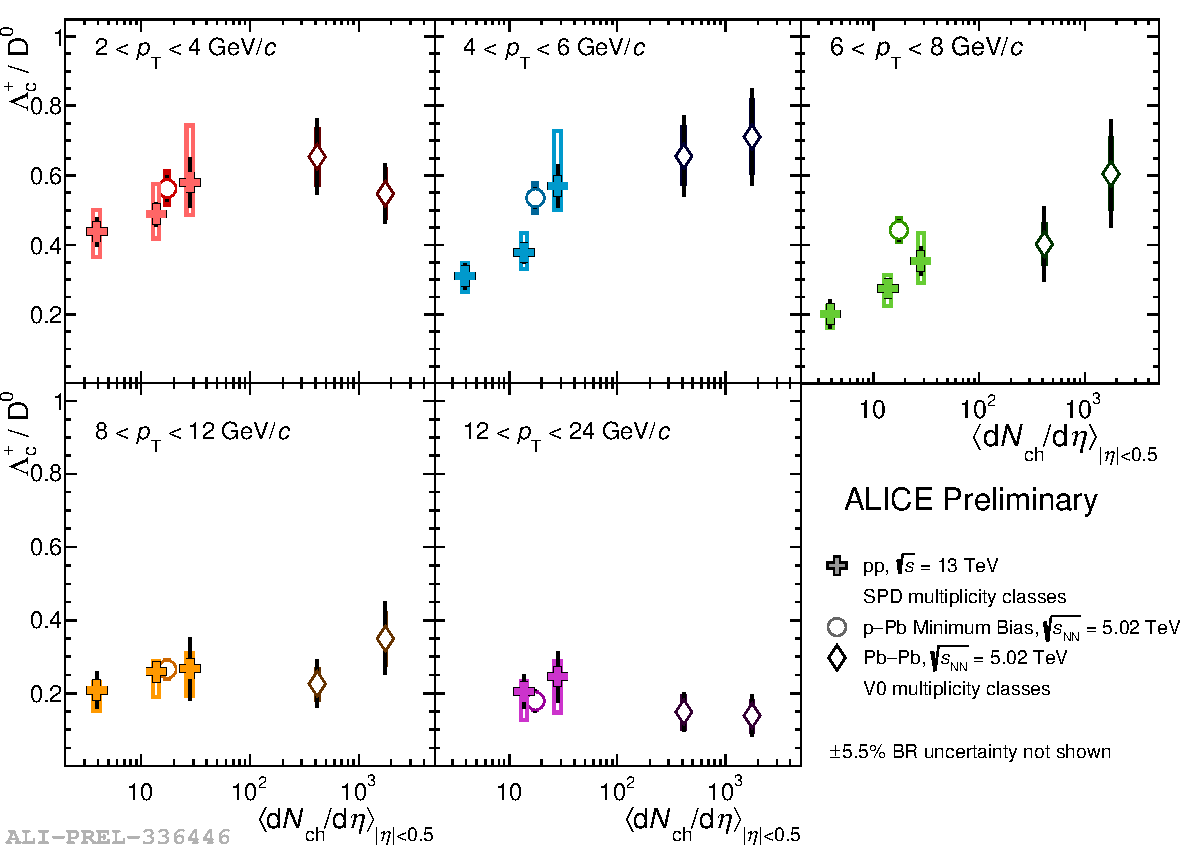
\includegraphics[width=0.9\textwidth]{Plots/ppHM/2019-10-31-2019-10-31-LcOverD0VsMult_pp_pPb_PbPb.pdf}
\caption{Alleluja}
\label{fig:LcDo_allsystems}
\end{figure}

\begin{figure}[h]
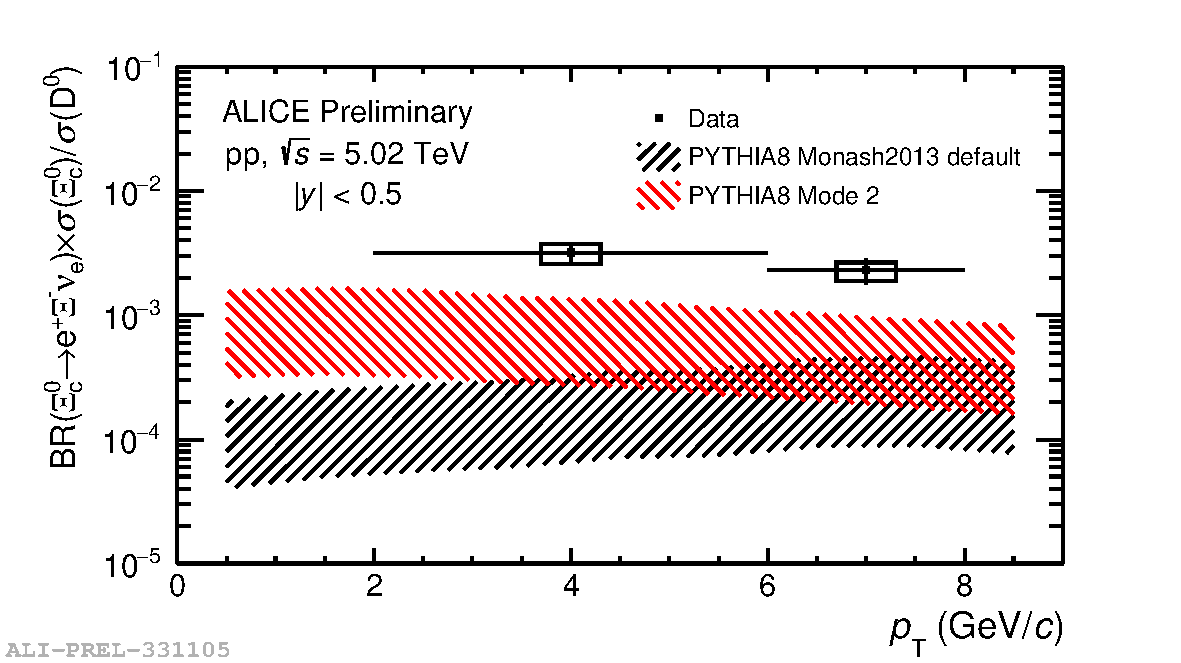
\includegraphics[width=0.49\textwidth]{Plots/Xi_c/2019-10-28-2019-10-28-Xic0toD0_5TeV_wModel1.pdf}
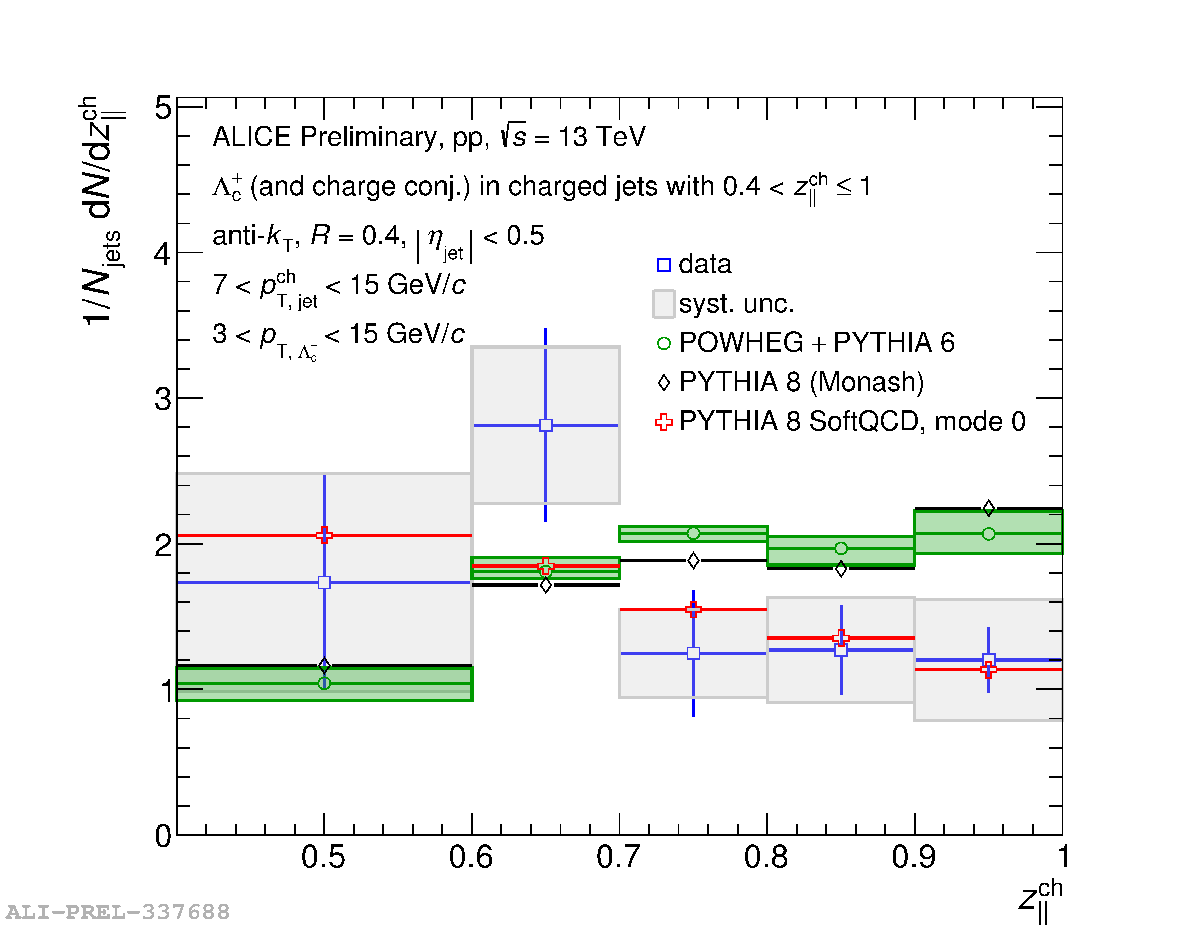
\includegraphics[width=0.49\textwidth]{Plots/FF/2019-10-31-finalwsys_wmodels_pt_jet_7_15.pdf}
\caption{Alleluja}
\label{fig:future}
\end{figure}

%% The Appendices part is started with the command \appendix;
%% appendix sections are then done as normal sections
%% \appendix

%% \section{}
%% \label{}

%% References
%%
%% Following citation commands can be used in the body text:
%% Usage of \cite is as follows:
%%   \cite{key}         ==>>  [#]
%%   \cite[chap. 2]{key} ==>> [#, chap. 2]
%%

%% References with BibTeX database:

\bibliographystyle{elsarticle-num}
\bibliography{<your-bib-database>}

%% Authors are advised to use a BibTeX database file for their reference list.
%% The provided style file elsarticle-num.bst formats references in the required Procedia style

%% For references without a BibTeX database:

% \begin{thebibliography}{00}

%% \bibitem must have the following form:
%%   \bibitem{key}...
%%

% \bibitem{}

% \end{thebibliography}

\end{document}

%%
%% End of file `nupha-template.tex'.
